
\documentclass[12pt]{article}
\usepackage[utf8]{inputenc}
\usepackage[T1]{fontenc}
\usepackage[spanish]{babel}
\usepackage{amsmath, amssymb}
\usepackage{geometry}
\usepackage{graphicx}
\usepackage{hyperref}
\geometry{margin=2.5cm}

\title{\textbf{Algoritmo BB84 de Distribución Cuántica de Claves}}
\author{Manuel Tagle, Patricio Palacios y Lukas Wolff}
\date{\today}

\begin{document}
\maketitle

El desarrollo realizado, asi como los codigos se encuentran en el siguiente \href{https://github.com/LukasWolff2002/T6_QUANTUM_MECHANICS}{link} a git hub.

\section{Bases de Codificación}
El protocolo utiliza dos bases ortogonales mutuamente incompatibles para representar los bits:
\begin{itemize}
    \item Base \textbf{Rectilínea (R)}: $\{|0\rangle, |1\rangle\}$, correspondiente a polarizaciones horizontal y vertical.
    \item Base \textbf{Diagonal (D)}: $\{|+\rangle, |-\rangle\}$, correspondiente a polarizaciones a $45^\circ$ y $135^\circ$.
\end{itemize}
Un mismo bit puede codificarse en diferentes bases, y si el receptor mide en la base incorrecta, el resultado será aleatorio.

\section{Parte 1: Sin intervención de Eve}
\subsection{Descripción del Proceso}
El protocolo sin presencia de un espía se desarrolla en los siguientes pasos:

\begin{enumerate}
    \item \textbf{Generación de secuencias por Alice:} genera $N$ bits aleatorios ($0$ o $1$) y $N$ bases aleatorias (R o D). Si es R y el bit es $0$, envía $|0\rangle$; si es R y el bit es $1$, envía $|1\rangle$; si es D y el bit es $0$, envía $|+\rangle$; si es D y el bit es $1$, envía $|-\rangle$.
    \item \textbf{Bob genera sus bases:} elige $N$ bases aleatorias para medir los qubits recibidos. Ahora bien
    \item \textbf{Bob mide:} compara sus bases con las de Alice. Si coinciden, conserva el bit; si no, lo descarta. Las combinaciones posibles son las siguientes:
    \begin{itemize}
        \item Alice R, Bob R: Bob obtiene el bit correcto.
        \item Alice R, Bob D: Bob obtiene un bit aleatorio (50\% de probabilidad de ser $0$ o $1$).
        \item Alice D, Bob R: Bob obtiene un bit aleatorio (50\% de probabilidad de ser $0$ o $1$).
        \item Alice D, Bob D: Bob obtiene el bit correcto.
        \item \textbf{Perdida de información:} en promedio, la mitad de los bits se descartan debido a la falta de coincidencia de bases, es decir, hay un $50\%$ de perdida de información, el cual tiene un $50\%$ de probabilidad de ser real, por lo tanto, se puede decir que hay un $25\%$ de perdida de información real. Aun asi, se descarta la mitad de los bits, logrando asi un Quantum Bit Error Rate (QBER) de $0\%$ en un canal ideal.
    \end{itemize}
    \item \textbf{Comparación de bases:} finalmente, Alice publica sus bases y Bob determina las coincidencias.
    \item \textbf{Extracción de clave cruda:} se seleccionan los bits correspondientes a bases coincidentes.
    \item \textbf{Verificación de errores:} Bob revela una pequeña fracción de la clave para comparar con Alice. Si los bits coinciden, la clave es válida.
\end{enumerate}

\subsection{Resultados Esperados}
Si el canal es ideal (sin ruido), la tasa de error cuántica o QBER (\textit{Quantum Bit Error Rate}) debería ser aproximadamente $0\%$.
La mitad de los bits se descartan debido a la falta de coincidencia de bases, resultando en una \textbf{clave cruda} de longitud cercana a $N/2$.

\section{Parte 2: Con intervención de Eve}
\subsection{Ataque de Interceptación y Reenvío}
En este escenario, un atacante (Eve) intercepta los qubits enviados por Alice, los mide en bases aleatorias y luego reenvía a Bob qubits codificados según sus propios resultados. 
El procedimiento es el siguiente:

\begin{enumerate}
    \item Eve genera sus bases aleatorias.
    \item Eve mide los qubits de Alice. Si su base coincide con la de Alice, obtiene el bit correcto; si no, el resultado es aleatorio.
    \item Eve reenvía a Bob los bits medidos, preparados en su base.
    \item Bob mide los qubits reenviados utilizando sus propias bases. Por lo cual se generan las siguientes combinaciones:
    \begin{itemize}
        \item Alice R, Eve R, Bob R: Bob obtiene el bit correcto.
        \item Alice R, Eve R, Bob D: Bob obtiene un bit aleatorio (50\% de acierto).
        \item Alice R, Eve D, Bob R: Bob obtiene un bit aleatorio (50\% de acierto).
        \item Alice R, Eve D, Bob D: Bob obtiene el bit correcto con 50\% de probabilidad.
        \item Alice D, Eve R, Bob R: Bob obtiene el bit correcto con 50\% de probabilidad. % <-- corregido
        \item Alice D, Eve R, Bob D: Bob obtiene un bit aleatorio (50\% de acierto).
        \item Alice D, Eve D, Bob R: Bob obtiene el bit correcto con 50\% de probabilidad.
        \item Alice D, Eve D, Bob D: Bob obtiene el bit correcto.
    \end{itemize}
\end{enumerate}

\subsection{Detección de la Presencia de Eve}
El intento de espionaje introduce perturbaciones detectables. Si Eve mide con una base incorrecta, perturba el estado original, 
de modo que cuando Bob mida (incluso con la base correcta), tiene un 50\% de probabilidad de obtener el bit erróneo.
El resultado es que la tasa de error esperada (\textbf{QBER}) se eleva aproximadamente a un \textbf{25\%}.


\section{Detección de la presencia de Eve y autenticación del canal clásico}

Es posible detectar la presencia de un espía (\textbf{Eve}) mediante la estimación de la 
\textbf{tasa de error cuántica} o \textbf{QBER} (\textit{Quantum Bit Error Rate}). 
Cuando Eve intenta interceptar y medir los fotones enviados por Alice, 
su medición altera los estados cuánticos originales debido al principio de indeterminación 
y al teorema de no clonación. Como consecuencia, Bob recibe un conjunto de bits con 
errores adicionales respecto a los de Alice.

Después de la transmisión, Alice y Bob comunican públicamente una muestra de sus bits 
por un \textbf{canal clásico}, comparando los resultados para estimar el QBER:

\[
QBER = \frac{N_{\text{errores}}}{N_{\text{bits\ evaluados}}}.
\]

Si el canal es ideal y no existe Eve, el QBER debería ser cercano a $0\%$.  
Sin embargo, si Eve realiza un ataque de \textit{interceptación y reenvío}, 
el valor esperado es aproximadamente $25\%$.

\subsubsection*{Entropía y límite del 11\%}

La capacidad de Alice y Bob para obtener una clave segura depende de la 
\textbf{entropía mutua} entre sus secuencias ($I_{AB}$) y la información potencial 
que Eve puede haber obtenido ($I_{AE}$).  
La condición de seguridad asintótica es:

\[
I_{AB} > I_{AE}.
\]

Utilizando el formalismo de Shannon, el contenido de información de un bit con 
probabilidad de error $e$ se expresa mediante la \textbf{entropía binaria}:

\[
H(e) = -e \log_2(e) - (1-e)\log_2(1-e).
\]

Durante la fase de \textit{amplificación de privacidad}, el número de bits seguros que pueden 
extraerse se aproxima por:

\[
R \approx 1 - 2H(QBER).
\]

Para que la clave final sea positiva ($R > 0$), se requiere que la entropía no supere un 
valor crítico. Resolviendo $1 - 2H(QBER) = 0$ se obtiene el umbral:

\[
QBER_{\text{máx}} \approx 0.1100 \ \text{(11\%)}.
\]

Por encima de este límite, la información que Eve podría haber adquirido supera la que 
Alice y Bob comparten de forma segura, haciendo imposible la generación de una clave secreta.  
Por debajo de este umbral, la información de Eve es menor que la correlación entre 
Alice y Bob, y por lo tanto la clave puede \textbf{purificarse} mediante corrección de errores 
y amplificación de privacidad.

En resumen, el protocolo BB84 es seguro si:

\[
QBER < 11\%.
\]

\subsection{Autenticación del Canal Clásico}

El canal clásico utilizado para la comunicación pública entre Alice y Bob no necesita ser 
confidencial, pero sí debe ser \textbf{autenticado}, es decir, debe garantizarse que los 
mensajes no puedan ser modificados ni falsificados por Eve.  
Si Eve pudiera alterar el canal clásico, podría introducir mensajes falsos o reemplazar 
los de Alice y Bob, rompiendo la integridad del protocolo.

La autenticación puede lograrse mediante \textbf{códigos de autenticación universales}, 
también conocidos como \textbf{Wegman--Carter MACs}.  
En este esquema, Alice y Bob comparten una corta clave secreta inicial $k$, y cada mensaje 
$m$ transmitido se acompaña de una etiqueta de autenticación $t = h_k(m)$, donde 
$h_k$ pertenece a una familia de funciones hash universales.  
Eve, sin conocer $k$, no puede generar una etiqueta válida para un mensaje falso.

Después de cada sesión de distribución cuántica, una pequeña fracción de la nueva clave 
se reserva para reemplazar la clave de autenticación $k$, asegurando así la continuidad 
del sistema sin necesidad de recurrir nuevamente a un canal precompartido.

En resumen:
\begin{itemize}
    \item La detección de Eve se realiza midiendo el QBER y verificando si excede el 11\%.
    \item El canal clásico debe ser autenticado para evitar ataques de suplantación o manipulación.
    \item La combinación de detección (entropía cuántica) y autenticación (seguridad clásica) 
          garantiza la inviolabilidad del protocolo BB84.
\end{itemize}

\section{Desarrollo del codigo}

Se desarrollo un codigo en Python que simula el protocolo BB84 tanto en la parte sin
intervención de Eve como en la parte con intervención de Eve. El código genera las
secuencias de bits y bases aleatorias para Alice, Bob y Eve (en el caso de Eve), 
realiza las mediciones correspondientes y calcula el QBER resultante.

\subsection{Caso sin intervención de Eve}

Luego de que ALice y Bob realizan el protocolo sin la intervención de Eve, se obtiene el siguiente resultado:

\begin{figure}
    \centering
    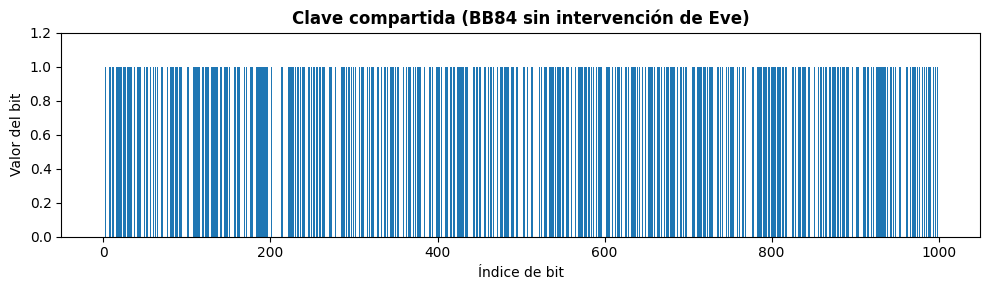
\includegraphics[width=0.9\textwidth]{caso_1.png}
    \caption{Resultados del protocolo BB84 sin intervención de Eve.}
\end{figure}

Donde se observa que el QBER es $0\%$, donde un $50\%$ de los bits son descartados
debido a la falta de coincidencia de bases entre Alice y Bob.

En el caso que hay una intervencion de Eve, se obtiene el siguiente resultado:

\begin{figure}
    \centering
    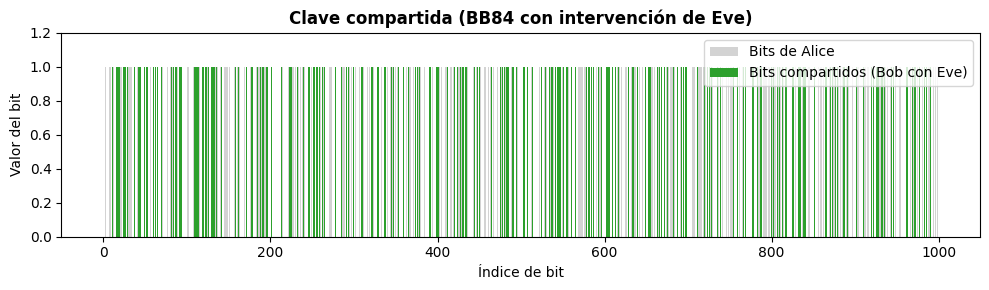
\includegraphics[width=0.9\textwidth]{caso_2.png}
    \caption{Resultados del protocolo BB84 con intervención de Eve.}
\end{figure}

Donde se observa que el QBER es aproximadamente $25\%$, lo que indica la presencia
de un espía en el canal de comunicación.

\end{document}


